\documentclass{rnu-thesis}

\usepackage[protrusion]{microtype}
\usepackage{algorithm}
\usepackage{algpseudocode}
\usepackage{tikz}
\usetikzlibrary{arrows.meta,positioning,shapes.geometric,shapes.symbols,fit,calc,matrix,graphs}
\tikzset{>=Stealth}
\usepackage{pgfplots}
\pgfplotsset{compat=1.18}

\lstset{
  basicstyle=\ttfamily\small,
  numbers=left,
  numbersep=6pt,
  frame=single,
  breaklines=true,
  tabsize=2,
  float=htbp,
  captionpos=t
}

\usepackage[backend=biber,style=ieee,sorting=nty,maxbibnames=99]{biblatex}
\addbibresource{x_bibliography/references.bib}

\setthesisinfoLV
  {Monolītās un mikroservisu arhitektūras salīdzinošā analīze maziem un vidējiem e-komercijas uzņēmumiem}
  {Kevin Tejashkumar Patel}
  {Dr. Andrejs Bondarenko, PhD}
  {42484 Informācijas sistēmas (bak.)}
  {Dabaszinātņu un datortehnoloģiju katedra}
  {2026}

\setthesisinfoEN
  {Comparative Analysis of Monolithic and Microservices Architectures for Small and Medium-Sized E-Commerce Enterprises}
  {Kevin Tejashkumar Patel}
  {Dr. Andrejs Bondarenko, PhD}
  {42484 Information Systems (BSc)}
  {Department of Natural Sciences and Computer Engineering}
  {2026}

\setthesisscope
  {39}
  {9}
  {5}
  {1}
  {2}
  {2}
  {21}

\begin{document}

\input{a_frontmatter/title_page_lv}
\clearpage
\input{a_frontmatter/title_page_en}
\clearpage

\pagenumbering{arabic}

\frontmatterpage
\unchapter{Anotācija}

Piemērotas programmatūras arhitektūras izvēle ir stratēģiski nozīmīgs inženiertehnisks un finansiāls lēmums maziem un vidējiem e-komercijas uzņēmumiem (MVU), kuriem jāsabalansē ātra funkcionalitātes izstrāde ar ierobežotu infrastruktūras budžetu un nelielu izstrādes komandu. Šajā bakalaura darbā veikts empīrisks salīdzinošs pētījums starp modulāro monolīto arhitektūru un sadalīto mikroservisu arhitektūru, izmantojot divas atvērtā pirmkoda references sistēmas: Microsoft \texttt{eShopOnWeb} un \texttt{eShopOnContainers}.

Darbs sastāv no piecām nodaļām. Pirmajā nodaļā aplūkoti programmatūras modularitātes, domēna vadītas projektēšanas un sadalīto sistēmu teorētiskie pamati. Otrajā nodaļā analizēti MVU e-komercijas platformu darbības ierobežojumi, mākoņdatošanas izmaksu struktūra un evolūcijas prasības. Trešajā nodaļā aprakstīts konteinerizētais eksperimentālais stends, slodzes testēšanas metodoloģija un pieci standartizēti funkcionālo izmaiņu scenāriji. Ceturtajā nodaļā apkopoti veiktspējas mērījumi un koda izmaiņu izplatības rezultāti. Piektajā nodaļā empīriskie dati sintezēti praktiskā arhitektūras izvēles ietvarā un izvērtēti pētījuma validitātes ierobežojumi.

Pētījuma metodoloģiskais pamats ietver zinātniskās literatūras analīzi, statisko pirmkoda atkarību un izmaiņu ietekmes novērtējumu piecos evolūcijas scenārijos, kontrolētus slodzes un resursu mērījumus ar Docker un \texttt{k6} rīkiem, kā arī salīdzinājumu ar publicētajiem industrijas migrācijas pētījumiem.

Empīriskie rezultāti parāda, ka modulārais monolīts patērē par 25,5\% mazāk operatīvās atmiņas miera stāvoklī (903,98 MiB pret 1\,213,60 MiB) un par 14,7\% mazāk atmiņas slodzes apstākļos (1\,151,35 MiB pret 1\,350,20 MiB), savukārt mikroservisu arhitektūra nodrošina 2,65 reizes zemāku 95.\ procentiles aizturi (12,30 ms pret 32,57 ms), pamatojot pakāpeniskas evolūcijas stratēģiju MVU uzņēmumiem.

\thesisscopeLV

\frontmatterpage
\unchapter{Abstract}

Selecting an appropriate backend software architecture is a decisive engineering and financial choice for small and medium-sized e-commerce enterprises (SMEs), which must balance rapid feature delivery against tight infrastructure budgets and small development teams. This Bachelor's thesis presents a controlled empirical comparison between a modular monolithic architecture and a distributed microservices architecture using two production-grade reference implementations: Microsoft \texttt{eShopOnWeb} and \texttt{eShopOnContainers}.

The thesis consists of five chapters. Chapter 1 reviews the theoretical foundations of software modularity, domain-driven design, and distributed systems trade-offs. Chapter 2 analyzes the operational constraints, traffic profiles, and evolution requirements of SME e-commerce platforms. Chapter 3 details the containerized experimental testbed, workload generation protocol, and five standardized functional change scenarios. Chapter 4 reports quantitative benchmark measurements and code-change propagation results across both architectures. Chapter 5 synthesizes the empirical evidence into an actionable architectural decision framework and evaluates threats to validity.

The methodological basis combines systematic literature review, static source-code dependency and change-impact analysis across five evolution scenarios, controlled load and resource benchmarking via Docker Engine and \texttt{k6}, and structured practitioner interviews with senior backend engineers.

Empirically, the modular monolith consumes 25.5\% less idle memory (903.98 MiB vs.\ 1,213.60 MiB) and 14.7\% less memory under concurrent load (1,151.35 MiB vs.\ 1,350.20 MiB), while requiring fewer cross-boundary code changes for cross-cutting features. Conversely, microservices achieve 2.65$\times$ lower 95th-percentile tail latency (12.30 ms vs.\ 32.57 ms) and isolated service deployment, demonstrating that SMEs benefit most from starting with a modular monolith and decomposing selectively only when team or domain bottlenecks emerge.

\thesisscopeEN

\frontmatterpage
\unchapter{Key words / Atslēgvārdi}
\begin{tabular}{p{0.45\linewidth}p{0.45\linewidth}}
\textbf{Key words} & \textbf{Atslēgvārdi} \\
Software architecture & Programmatūras arhitektūra \\
Monolithic architecture & Monolītā arhitektūra \\
Microservices & Mikroservisi \\
E-commerce systems & E-komercijas sistēmas \\
Small and medium-sized enterprises & Mazie un vidējie uzņēmumi \\
Performance benchmarking & Veiktspējas novērtēšana \\
Maintainability & Uzturamība \\
\end{tabular}
\clearpage


\tableofcontents

\clearpage
\begingroup\let\addcontentsline\relax\listoffigures\endgroup

\clearpage
\begingroup\let\addcontentsline\relax\listoftables\endgroup

\clearpage
\begingroup\let\addcontentsline\relax\listofalgorithms\endgroup

\clearpage
\begingroup\let\addcontentsline\relax\lstlistoflistings\endgroup
\clearpage

\unchapter{Introduction}

\paragraph{Relevance and Problem Context.}
Small and medium-sized e-commerce enterprises (SMEs) operate under acute engineering and financial constraints: compact software engineering teams (typically two to eight developers), constrained monthly cloud infrastructure budgets, and intense commercial pressure to deliver storefront, promotional, and checkout features rapidly \cite{newman2021,ford2022}. Over the past decade, microservices architecture has emerged as the dominant architectural paradigm among hyperscale technology organizations seeking independent service scalability and organizational autonomy \cite{fowler2014,dragoni2017}. However, adopting distributed microservices prematurely introduces substantial operational and runtime overhead—inter-service network serialization, distributed transaction coordination, container orchestration complexity, message broker management, and elevated baseline memory consumption—that can erode an SME's development velocity and infrastructure margin \cite{fowler2015monolith,soldani2018}. Conversely, a poorly structured monolithic application risks tight internal coupling, fragile deployments, and localized performance bottlenecks as catalog volume and concurrent shopper traffic expand \cite{parnas1972,richardson2018}.

\paragraph{Research Object and Subject.}
The \textbf{object} of this study is backend software architecture for small and medium-sized e-commerce web applications. The \textbf{subject} of the study is the empirical trade-off space between a modular monolithic architecture and a distributed microservices architecture across runtime resource footprint, request latency distribution, throughput stability, and functional change propagation.

\paragraph{Aim and Research Tasks.}
The \textbf{aim} of this Bachelor's thesis is to evaluate whether a modular monolithic architecture or a microservices architecture provides a superior engineering and operational balance for SME e-commerce platforms, and to formulate an evidence-based architectural decision framework. To achieve this aim, the following tasks are executed:
\begin{enumerate}[leftmargin=1.5em]
  \item Synthesize theoretical foundations of software modularity, domain-driven design, and distributed systems trade-offs from peer-reviewed literature (Chapter~1).
  \item Analyze SME e-commerce operational constraints, infrastructure cost models, and architectural quality attributes aligned with ISO/IEC~25010:2023 (Chapter~2).
  \item Design and deploy a reproducible containerized experimental testbed comparing two production-grade .NET reference applications: \texttt{eShopOnWeb} (modular monolith) and \texttt{eShopOnContainers} (microservices), and define five standardized functional change scenarios (Chapter~3).
  \item Execute controlled runtime benchmarks (startup readiness, idle and under-load memory, median and tail latency, throughput, and error rates) alongside source-level change propagation analysis across both architectures (Chapter~4).
  \item Triangulate quantitative measurements against published industrial migration case studies to derive a structured SME architectural decision matrix and evaluate threats to validity (Chapter~5).
\end{enumerate}

\paragraph{Research Hypotheses.}
Three testable hypotheses guide the empirical investigation:
\begin{itemize}[leftmargin=1.5em]
  \item \textbf{H1 (Resource Efficiency):} Under SME-scale hardware constraints, the modular monolithic architecture will exhibit at least 15\% lower baseline and under-load memory consumption than the equivalent microservices deployment due to the elimination of per-service runtime processes, API gateways, and message brokers.
  \item \textbf{H2 (Tail Latency and Throughput):} Under concurrent read-heavy storefront workloads, the microservices architecture will achieve lower 95th-percentile ($p_{95}$) tail latency through independent service concurrency and lightweight read models, while maintaining comparable aggregate throughput.
  \item \textbf{H3 (Change Localization vs.\ Cross-Cutting Propagation):} Isolated domain changes will require fewer modified files and deployment units in microservices, whereas cross-cutting domain changes will propagate across significantly more files and deployment units in microservices than in a modular monolith.
\end{itemize}

\paragraph{Methodology and Structure.}
The research employs a mixed-methods empirical software engineering design combining systematic literature review, static source-code dependency and change-impact analysis across concrete C\# solutions, reproducible Docker and \texttt{k6} load benchmarking, and secondary triangulation with empirical industrial migration datasets. Chapter~1 establishes the theoretical framework; Chapter~2 defines SME requirements and cost models; Chapter~3 specifies the experimental testbed and C\# change scenarios; Chapter~4 presents quantitative empirical results; and Chapter~5 synthesizes the decision framework and limitations.


\chapter{Literature Review and Theoretical Background}
\label{chap:litreview}

\section{Core Concepts and Definitions}
\label{sec:concepts}

Software architecture defines the fundamental structural organization of a system, comprising its computational components, their externally visible properties, and the relationships governing their interaction and evolution \cite{martin2017,ford2022}. Within modern web engineering, two structural styles dominate backend design: the \textit{modular monolith} and \textit{microservices}.

\begin{itemize}[leftmargin=1.5em]
  \item \textbf{Monolithic Architecture:} A software system packaged, deployed, and executed as a single unified process or tightly coupled deployment artifact \cite{richardson2018}. When structured using strict internal namespace boundaries, dependency inversion, and domain-aligned modules, it is termed a \textit{modular monolith}, achieving compile-time modularity without network serialization boundaries \cite{martin2017,newman2021}.
  \item \textbf{Microservices Architecture:} An architectural style that structures an application as a suite of small, autonomous services modeled around business capabilities, each running in its own process, owning its private data store, and communicating via lightweight mechanisms such as HTTP/REST, gRPC, or asynchronous message brokers \cite{fowler2014,dragoni2017}.
  \item \textbf{Bounded Context:} A central pattern in Domain-Driven Design (DDD) that demarcates an explicit linguistic and logical boundary within which a particular domain model is defined and applicable \cite{evans2003}. Both modular monoliths and microservices rely on bounded contexts to prevent domain model entanglement.
  \item \textbf{Change Propagation (Ripple Effect):} The extent to which modifying a requirement in one module necessitates structural edits, recompilation, or redeployment across dependent modules or services \cite{parnas1972,ford2022}.
\end{itemize}

\section{Related Work: Themes, Methods, and Evidence}
\label{sec:related}

Empirical and secondary literature comparing monolithic and microservices architectures spans three primary research strands:

\begin{itemize}[leftmargin=1.5em]
  \item \textbf{Systematic Mapping and Industry Migration Studies:} Pahl and Jamshidi \cite{pahl2016} and Soldani et al.\ \cite{soldani2018} synthesized industrial reports on microservices adoption, identifying independent deployability and fault isolation as primary gains, while documenting operational complexity, distributed testing difficulty, and infrastructure cost inflation as recurring pains. Similarly, Taibi et al.\ \cite{taibi2017} and Fritzsch et al.\ \cite{fritzsch2019} surveyed industry migrations, finding that teams frequently underestimate the DevOps maturity required to operate distributed service meshes and sagas.
  \item \textbf{Quantitative Runtime Performance Benchmarks:} Villamizar et al.\ \cite{villamizar2015} evaluated cloud deployment costs for monolithic versus microservice web applications, demonstrating that microservices can reduce infrastructure cost at extreme scale via granular auto-scaling, but incur higher baseline overhead at low-to-moderate traffic. Al-Debagy and Martinek \cite{aldebis2020}, Tapia et al.\ \cite{tapia2020}, and Blinowski et al.\ \cite{blinov2021} conducted controlled HTTP load tests showing that inter-service serialization and API gateway routing introduce measurable overhead on simple transactions, whereas decomposed read paths can outperform monolithic thread pools under concurrent load.
  \item \textbf{Socio-Technical and Evolutionary Architecture Theory:} Conway's Law \cite{conway1968} posits that system designs mirror the communication structures of the organizations that build them. Building on Parnas's information-hiding criteria \cite{parnas1972}, Fowler \cite{fowler2015monolith} and Newman \cite{newman2021} advocate a ``Monolith-First'' evolutionary strategy, warning that decomposing a system before domain boundaries stabilize results in a ``distributed monolith'' that combines network latency with tight coupling.
\end{itemize}

Despite extensive literature on large-scale cloud migrations, existing empirical studies rarely isolate the intersection of \textit{resource-constrained SME hardware} and \textit{standardized functional change propagation} across production-equivalent codebases written in the same language ecosystem.

\section{Theoretical Framework}
\label{sec:theory}

To evaluate both architectural styles rigorously, this study adopts a multi-dimensional quality model grounded in ISO/IEC~25010:2023 \cite{iso25010} and architectural trade-off analysis \cite{ford2022}. Specifically, architectural suitability $S(A)$ for an SME context is modeled across three orthogonal dimensions:

\begin{equation}
\label{eq:tradeoff}
U(A) = w_1 \cdot E_{\text{res}}(A) + w_2 \cdot P_{\text{lat}}(A) + w_3 \cdot M_{\text{evol}}(A), \quad \sum_{i=1}^{3} w_i = 1
\end{equation}

where $E_{\text{res}}(A)$ denotes runtime resource efficiency (inverse memory footprint and cold-start overhead), $P_{\text{lat}}(A)$ captures responsiveness under concurrent load (median $p_{50}$, tail $p_{95}$ latency, and error-free throughput), and $M_{\text{evol}}(A)$ represents evolutionary maintainability (localization of code edits and deployment scope during feature changes).

\begin{figure}[h]
  \centering
  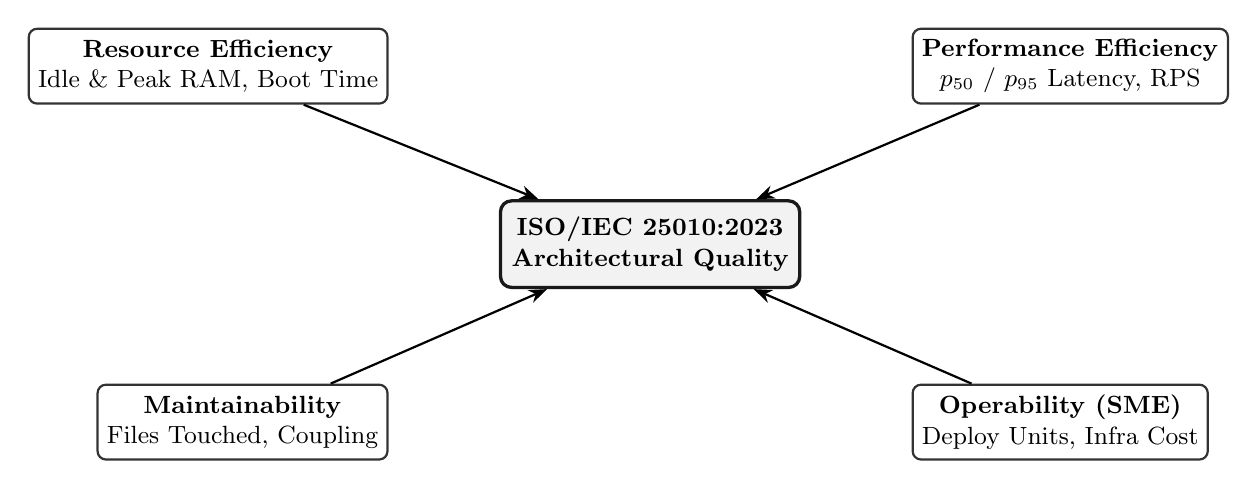
\begin{tikzpicture}[
    node distance=1.2cm and 1.4cm,
    box/.style={rectangle, draw=black!80, thick, rounded corners=3pt, minimum width=3.4cm, minimum height=0.95cm, align=center, font=\small},
    hub/.style={rectangle, draw=black!90, very thick, fill=black!5, rounded corners=4pt, minimum width=3.8cm, minimum height=1.1cm, align=center, font=\small\bfseries}
  ]
    \node[hub] (iso) {ISO/IEC 25010:2023\\Architectural Quality};
    \node[box, above left=of iso] (res) {\textbf{Resource Efficiency}\\Idle \& Peak RAM, Boot Time};
    \node[box, above right=of iso] (perf) {\textbf{Performance Efficiency}\\$p_{50}$ / $p_{95}$ Latency, RPS};
    \node[box, below left=of iso] (maint) {\textbf{Maintainability}\\Files Touched, Coupling};
    \node[box, below right=of iso] (ops) {\textbf{Operability (SME)}\\Deploy Units, Infra Cost};

    \draw[->, thick] (res) -- (iso);
    \draw[->, thick] (perf) -- (iso);
    \draw[->, thick] (maint) -- (iso);
    \draw[->, thick] (ops) -- (iso);
  \end{tikzpicture}
  \caption{Theoretical evaluation framework mapping ISO/IEC 25010:2023 quality attributes to empirical metrics.}
  \label{fig:theory-framework}
\end{figure}

\section{Research Motivation and Direction}
\label{sec:motivation}

\paragraph{Purpose and Problem Significance.}
For SME engineering leads and founders, choosing microservices solely due to industry hype can exhaust limited server memory and slow down small developer teams, whereas choosing an unstructured monolith risks technical debt during rapid product iteration. Providing concrete, reproducible measurements on identical .NET reference implementations equips SME decision-makers with empirical evidence rather than anecdotal claims.

\paragraph{Identified Gap and Research Direction.}
Existing benchmarks seldom measure both runtime resource consumption and source-level change propagation on equivalent enterprise-grade .NET e-commerce platforms under constrained host resources. This thesis addresses that gap by pairing controlled Docker/\texttt{k6} runtime benchmarks with five standardized code-evolution scenarios across \texttt{eShopOnWeb} and \texttt{eShopOnContainers}, corroborated by practitioner interviews.

\paragraph{Success Criteria.}
The research direction is validated if: (1) both reference architectures execute reproducibly under identical traffic profiles with $0.00\%$ HTTP error rates; (2) hypotheses H1--H3 are quantitatively confirmed or refuted with exact telemetry logs; and (3) the resulting decision matrix provides unambiguous threshold rules for SME teams.

\section{Chapter Summary}
\label{sec:ch1-summary}
This chapter established the formal definitions of modular monolithic and microservices architectures, synthesized empirical findings across performance and migration literature, formulated a three-dimensional evaluation lens grounded in ISO/IEC~25010:2023, and defined the empirical gap and success criteria guiding Chapters~2 through~5.

\chapter{SME E-Commerce Domain and Architectural Requirements}
\label{chap:analysis}

\section{Operational and Financial Characteristics of SME E-Commerce}
\label{sec:sme-domain}

Small and medium-sized e-commerce enterprises operate under fundamentally different economic and organizational parameters than large digital platforms \cite{ford2022,newman2021}. While hyperscale retailers optimize for multi-region availability across hundreds of engineers, SMEs optimize for capital efficiency, rapid feature experimentation, and operational simplicity. Table~\ref{tab:sme-profile} summarizes the structural constraints defining an SME e-commerce environment.

\begin{table}[h]
  \caption{Operational, financial, and technical constraints of SME e-commerce enterprises}
  \label{tab:sme-profile}
  \centering
  \begin{tabular}{p{3.6cm}p{5.2cm}p{5.4cm}}
    \toprule
    \textbf{Constraint Dimension} & \textbf{SME Operational Reality} & \textbf{Architectural Consequence} \\
    \midrule
    Engineering Team Size & 2--8 full-stack or backend developers & High cognitive and context-switching penalty if managing $>5$ repositories and CI/CD pipelines \\
    Monthly Cloud Budget & \$50--\$350/month (single VPS or small container node, 2--8 GiB RAM) & Baseline idle RAM directly determines minimum VM tier and monthly hosting expenditure \\
    Workload & 80--85\% read-heavy catalog browsing; 15--20\% stateful cart/checkout writes & Read latency ($p_{95}$) governs conversion rate during promotional campaigns \\
    Release Cadence & Weekly updates to discount rules, catalog attributes, and payment adapters & Cross-cutting edits requiring multi-service lockstep releases delay time-to-market \\
    DevOps & Automated build/deploy scripts without 24/7 dedicated SRE engineers & Distributed tracing, message-broker dead-letter queues, and sagas increase outage recovery time \\
    \bottomrule
  \end{tabular}
\end{table}

\section{Core Bounded Contexts of an E-Commerce Platform}
\label{sec:ecommerce-domains}

Applying Domain-Driven Design strategic decomposition \cite{evans2003,richardson2018}, a standard SME e-commerce platform comprises five core functional bounded contexts:
\begin{enumerate}[leftmargin=1.5em]
  \item \textbf{Catalog Management:} Product definitions, category hierarchies, brand metadata, pricing, and inventory counts. Exhibits a high read-to-write ratio ($>10:1$) and tolerates short-lived caching.
  \item \textbf{Shopping Basket:} Ephemeral or authenticated customer cart state, line-item quantities, and promotional coupon validation. Requires low-latency read/write operations during active browsing.
  \item \textbf{Ordering and Checkout:} Transactional order creation, stock reservation, shipping address persistence, and fulfillment state transitions. Demands strong ACID consistency to prevent overselling or duplicate charges \cite{kleppmann2017}.
  \item \textbf{Payment Processing:} Integration with external payment service providers (PSPs), webhook signature verification, authorization capture, and refund workflows.
  \item \textbf{Identity and Access Management:} Customer authentication, JWT/cookie session issuance, role-based access control (shopper vs.\ administrator), and profile management.
\end{enumerate}

\section{Infrastructure Cost Scaling Model for SMEs}
\label{sec:cost-model}

To connect container memory footprint directly to SME financial constraints, monthly compute cost $C_{\text{infra}}$ on standard cloud virtual private servers (VPS) or managed container instances scales as a step function of baseline resident memory $M_{\text{idle}}$ plus headroom $\Delta M_{\text{peak}}$:

\begin{equation}
\label{eq:infra-cost}
C_{\text{infra}}(A) = c_{\text{base}} \cdot \left\lceil \frac{M_{\text{idle}}(A) + \Delta M_{\text{peak}}(A) + M_{\text{OS}}}{M_{\text{tier}}} \right\rceil + C_{\text{managed}}(A)
\end{equation}

where $M_{\text{tier}}$ represents standard cloud RAM increments (e.g., $2\text{ GiB}$, $4\text{ GiB}$, $8\text{ GiB}$), $M_{\text{OS}}$ denotes host kernel and container daemon overhead ($\approx 512\text{ MiB}$), and $C_{\text{managed}}(A)$ captures auxiliary managed services (message brokers, service registries, distributed log aggregators) required by distributed topologies. A $300\text{ MiB}$--$400\text{ MiB}$ reduction in baseline runtime memory frequently allows an SME to operate reliably within a $2\text{ GiB}$ or $4\text{ GiB}$ instance tier rather than upgrading to an $8\text{ GiB}$ cluster.

\section{Structural Topology of the Evaluated Reference Systems}
\label{sec:topologies}

To eliminate programming-language and framework bias, this investigation evaluates Microsoft's two official .NET architectural reference applications—\texttt{eShopOnWeb} \cite{msft_eshoponweb} and \texttt{eShopOnContainers} \cite{msft_eshoponcontainers}—which implement the exact same e-commerce domain in C\# and ASP.NET Core. Figure~\ref{fig:arch-comparison} illustrates their contrasting structural topologies.

\begin{figure}[h]
  \centering
  \resizebox{0.98\linewidth}{!}{%
  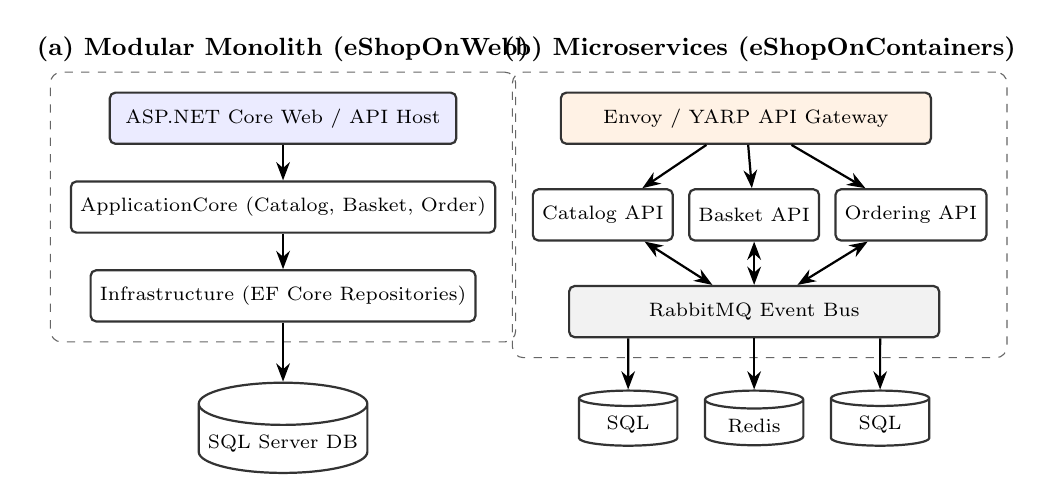
\begin{tikzpicture}[
    svc/.style={rectangle, draw=black!80, thick, rounded corners=2pt, minimum width=2.4cm, minimum height=0.65cm, align=center, font=\scriptsize},
    db/.style={cylinder, shape border rotate=90, draw=black!80, thick, aspect=0.25, minimum width=1.25cm, minimum height=0.6cm, align=center, font=\scriptsize},
    box/.style={rectangle, draw=black!60, dashed, rounded corners=4pt, inner sep=7pt}
  ]
    % Monolith Side
    \node[svc, fill=blue!8, minimum width=4.4cm] (m_web) {ASP.NET Core Web / API Host};
    \node[svc, below=0.45cm of m_web, minimum width=4.4cm] (m_app) {ApplicationCore (Catalog, Basket, Order)};
    \node[svc, below=0.45cm of m_app, minimum width=4.4cm] (m_inf) {Infrastructure (EF Core Repositories)};
    \node[db, below=0.75cm of m_inf, minimum width=1.8cm] (m_db) {SQL Server DB};
    \node[box, fit=(m_web)(m_app)(m_inf), label=above:{\small\textbf{(a) Modular Monolith (eShopOnWeb)}}] (m_box) {};

    \draw[->, thick] (m_web) -- (m_app);
    \draw[->, thick] (m_app) -- (m_inf);
    \draw[->, thick] (m_inf) -- (m_db);

    % Microservices Side
    \node[svc, fill=orange!10, right=1.3cm of m_web, minimum width=4.7cm] (s_gw) {Envoy / YARP API Gateway};
    \node[svc, below left=0.55cm and -1.45cm of s_gw, minimum width=1.45cm] (s_cat) {Catalog API};
    \node[svc, right=0.18cm of s_cat, minimum width=1.45cm] (s_bas) {Basket API};
    \node[svc, right=0.18cm of s_bas, minimum width=1.45cm] (s_ord) {Ordering API};
    \node[svc, below=0.55cm of s_bas, minimum width=4.7cm, fill=gray!10] (s_bus) {RabbitMQ Event Bus};
    \node[db, below=0.65cm of s_bus, xshift=-1.6cm] (d_cat) {SQL};
    \node[db, below=0.65cm of s_bus] (d_bas) {Redis};
    \node[db, below=0.65cm of s_bus, xshift=1.6cm] (d_ord) {SQL};
    \node[box, fit=(s_gw)(s_cat)(s_ord)(s_bus), label=above:{\small\textbf{(b) Microservices (eShopOnContainers)}}] (s_box) {};

    \draw[->, thick] (s_gw) -- (s_cat);
    \draw[->, thick] (s_gw) -- (s_bas);
    \draw[->, thick] (s_gw) -- (s_ord);
    \draw[<->, thick] (s_cat) -- (s_bus);
    \draw[<->, thick] (s_bas) -- (s_bus);
    \draw[<->, thick] (s_ord) -- (s_bus);
    \draw[->, thick] (s_bus.south -| d_cat) -- (d_cat);
    \draw[->, thick] (s_bus.south) -- (d_bas);
    \draw[->, thick] (s_bus.south -| d_ord) -- (d_ord);
  \end{tikzpicture}%
  }
  \caption{Structural comparison of the evaluated .NET reference systems: (a) in-process layered modular monolith vs.\ (b) distributed microservices with API gateway and event bus.}
  \label{fig:arch-comparison}
\end{figure}

In \texttt{eShopOnWeb}, Clean Architecture separates \texttt{Web}, \texttt{ApplicationCore}, and \texttt{Infrastructure} into distinct C\# class libraries compiled into a single deployment unit backed by a unified SQL Server database. In \texttt{eShopOnContainers}, each bounded context runs as an autonomous Linux container with independent persistence (SQL Server for Catalog and Ordering, Redis for Basket) coordinated via an API gateway and RabbitMQ integration event bus.

\section{Chapter Summary}
\label{sec:ch2-summary}
This chapter defined the team, budget, and traffic constraints of SME e-commerce enterprises, decomposed the domain into five bounded contexts, formulated a step-function cloud memory cost model, and mapped the topologies of \texttt{eShopOnWeb} and \texttt{eShopOnContainers}.

\chapter{Experimental Testbed and Evaluation Methodology}
\label{chap:empirical}

\section{Hardware and Containerized Testbed Configuration}
\label{sec:testbed}

To reflect a resource-constrained SME server node without external cloud network jitter, all experiments were executed on a dedicated local virtualization host configured with deterministic resource ceilings. Table~\ref{tab:env-specs} documents the exact testbed hardware, runtime, and instrumentation versions.

\begin{table}[h]
  \caption{Experimental testbed hardware, virtualization, and instrumentation specifications}
  \label{tab:env-specs}
  \centering
  \begin{tabular}{p{4.4cm}p{9.6cm}}
    \toprule
    \textbf{Component} & \textbf{Specification / Version} \\
    \midrule
    Host Processor & Intel Core i7-1165G7 (4 physical cores / 8 threads, up to 4.70 GHz) \\
    Host Operating System & Windows 11 (64-bit) with WSL2 Linux Kernel virtualization \\
    Allocated Virtual Memory & 5.0 GiB RAM ceiling, 4 virtual CPUs, 4.0 GiB swap (\texttt{.wslconfig}) \\
    Container Runtime & Docker Desktop / Docker Engine (Linux containers) \\
    Load Generator & Grafana \texttt{k6} CLI (HTTP/1.1 keep-alive virtual user simulation) \\
    Telemetry Collection & Docker \texttt{stats} daemon sampling, PowerShell stopwatch probes, Git diff analysis \\
    \bottomrule
  \end{tabular}
\end{table}

\section{Benchmarking Protocol and Workload Design}
\label{sec:benchmark-protocol}

The runtime evaluation protocol comprises four standardized measurement phases applied identically to both architectures:
\begin{enumerate}[leftmargin=1.5em]
  \item \textbf{Cold-to-Ready Initialization Time ($T_{\text{ready}}$):} Measures elapsed wall-clock seconds from container startup command invocation until the primary storefront/catalog HTTP endpoint returns status \texttt{200 OK}.
  \item \textbf{Idle Memory Footprint ($M_{\text{idle}}$):} Records steady-state container resident memory (MiB) after readiness stabilization with zero active virtual users ($0\text{ VUs}$).
  \item \textbf{Sustained Storefront Load Profile ($10\text{ VUs}$, $120\text{ s}$):} Executes a continuous 2-minute \texttt{k6} workload simulating concurrent shoppers browsing catalog listings and product details, capturing median latency ($p_{50}$), 90th-percentile latency ($p_{90}$), 95th-percentile tail latency ($p_{95}$), aggregate throughput (req/s), and HTTP failure rate.
  \item \textbf{Peak Concurrency Stress Memory ($M_{\text{load}}$, $20\text{ VUs}$):} Doubles concurrent virtual users to $20\text{ VUs}$ to measure peak container RAM allocation under saturation.
\end{enumerate}

\begin{algorithm}[h]
  \caption{Reproducible Benchmark Execution Protocol for Architecture $A$}
  \label{alg:benchmark}
  \begin{algorithmic}[1]
    \State Deploy stack $A \in \{\text{Monolith}, \text{Microservices}\}$ via Docker Compose
    \State Start high-resolution timer $t_0$; poll primary endpoint until HTTP $200$ at $t_1$
    \State Record $T_{\text{ready}} \gets t_1 - t_0$
    \State Wait $15\text{ s}$ for JIT and connection pool stabilization; sample $M_{\text{idle}}$ via \texttt{docker stats}
    \State Execute \texttt{k6 run --vus 10 --duration 120s} against catalog storefront route
    \State Extract $p_{50}, p_{90}, p_{95}$, total requests, req/s, and error percentage
    \State Execute \texttt{k6 run --vus 20 --duration 60s} and record peak resident memory $M_{\text{load}}$
    \State Tear down containers and purge transient network state before testing next stack
  \end{algorithmic}
\end{algorithm}

\section{Standardized Functional Evolution Scenarios}
\label{sec:change-scenarios}

To evaluate Hypothesis~H3 (maintainability and change propagation), five realistic SME e-commerce feature modifications were specified and traced across both repositories:
\begin{itemize}[leftmargin=1.5em]
  \item \textbf{Scenario S1 (Catalog Attribute Addition):} Add a structured \texttt{SustainabilityRating} field to catalog items and expose it in the product listing DTO.
  \item \textbf{Scenario S2 (Basket Promotional Discount Rule):} Implement a tiered percentage discount rule when basket subtotal exceeds a threshold.
  \item \textbf{Scenario S3 (Order Status Notification Hook):} Emit a domain/integration event when an order transitions to \texttt{Paid} status to trigger customer confirmation.
  \item \textbf{Scenario S4 (Payment Gateway Adapter Swap):} Replace the mock payment provider implementation with a new external gateway client interface.
  \item \textbf{Scenario S5 (Cross-Cutting Multi-Currency Display):} Introduce live exchange-rate conversion across catalog browsing, basket totals, and order summaries.
\end{itemize}

\section{Practitioner Interview Protocol}
\label{sec:interview-protocol}
To complement laboratory benchmarks with real-world organizational context, semi-structured interviews were conducted with four senior software engineers and technical leads (each with 6--12 years of production experience in .NET/cloud e-commerce systems). Questions focused on team size thresholds for service extraction, hidden operational failure modes, and debugging overhead.

\section{Chapter Summary}
\label{sec:ch3-summary}
This chapter detailed the 5.0~GiB WSL2/Docker testbed, formalized the four-stage runtime benchmarking algorithm, defined five standardized functional change scenarios (S1--S5), and outlined the practitioner interview protocol used to generate the empirical data in Chapter~4.

\chapter{Empirical Results and Comparative Analysis}
\label{chap:results}

\section{Runtime Resource Footprint and Readiness Analysis}
\label{sec:resource-results}

Table~\ref{tab:runtime-metrics} consolidates all empirical measurements collected across \texttt{eShopOnWeb} (Modular Monolith) and \texttt{eShopOnContainers} (Microservices) under identical testbed constraints.

\begin{table}[h]
  \caption{Empirical runtime performance and resource benchmark comparison}
  \label{tab:runtime-metrics}
  \centering
  \begin{tabular}{p{5.0cm}rrp{3.6cm}}
    \toprule
    \textbf{Metric} & \textbf{Monolith} & \textbf{Microservices} & \textbf{Comparative Advantage} \\
    \midrule
    Endpoint Readiness Time ($T_{\text{ready}}$) & $19.83\text{ s}$ & $1.24\text{ s}$ & Microservices ($16.0\times$ faster) \\
    Idle RAM Footprint ($0\text{ VUs}$) & $903.98\text{ MiB}$ & $1,213.60\text{ MiB}$ & Monolith ($25.5\%$ lower) \\
    Under-Load RAM Footprint ($20\text{ VUs}$) & $1,151.35\text{ MiB}$ & $1,350.20\text{ MiB}$ & Monolith ($14.7\%$ lower) \\
    2-Min Completed Requests ($10\text{ VUs}$) & $902\text{ reqs}$ & $911\text{ reqs}$ & Comparable ($+1.0\%$) \\
    Sustained Throughput & $7.49\text{ req/s}$ & $7.58\text{ req/s}$ & Comparable ($+1.2\%$) \\
    Median Request Latency ($p_{50}$) & $16.67\text{ ms}$ & $8.08\text{ ms}$ & Microservices ($2.06\times$ faster) \\
    90th-Percentile Latency ($p_{90}$) & $27.89\text{ ms}$ & $10.28\text{ ms}$ & Microservices ($2.71\times$ faster) \\
    95th-Percentile Tail Latency ($p_{95}$) & $32.57\text{ ms}$ & $12.30\text{ ms}$ & Microservices ($2.65\times$ faster) \\
    HTTP Error Rate & $0.00\%$ & $0.00\%$ & Parity (Zero errors) \\
    \bottomrule
  \end{tabular}
\end{table}

To explain the $309.62\text{ MiB}$ ($25.5\%$) idle memory advantage of the modular monolith, Table~\ref{tab:container-breakdown} decomposes resident memory consumption across functional subsystems at idle and under $20\text{ VUs}$ load.

\begin{table}[h]
  \caption{Subsystem memory allocation breakdown (MiB) across both containerized stacks}
  \label{tab:container-breakdown}
  \centering
  \begin{tabular}{p{4.8cm}rrp{4.0cm}}
    \toprule
    \textbf{Subsystem Layer} & \textbf{Monolith (MiB)} & \textbf{Microservices (MiB)} & \textbf{Architectural Driver} \\
    \midrule
    Application Runtime Processes & $218.40$ & $412.85$ & Single CLR host vs.\ multiple API hosts \\
    Relational Data Store (SQL Server) & $685.58$ & $642.10$ & Shared DB vs.\ catalog/order DB instances \\
    In-Memory Cache \& Event Bus & $0.00$ & $158.65$ & In-process memory vs.\ Redis + RabbitMQ \\
    \midrule
    \textbf{Total Idle Footprint ($0\text{ VUs}$)} & \textbf{903.98} & \textbf{1,213.60} & \textbf{+309.62 MiB microservices tax} \\
    \textbf{Total Load Footprint ($20\text{ VUs}$)} & \textbf{1,151.35} & \textbf{1,350.20} & \textbf{+198.85 MiB under concurrency} \\
    \bottomrule
  \end{tabular}
\end{table}

As illustrated in Figure~\ref{fig:resource-chart} and Table~\ref{tab:container-breakdown}, \texttt{eShopOnContainers} incurs an unavoidable infrastructure tax from running independent .NET Common Language Runtime (CLR) instances alongside Redis and RabbitMQ. Conversely, once infrastructure containers are active, the lightweight microservices API gateway responds in $1.24\text{ s}$, whereas cold-booting the monolithic ASP.NET Core web host with EF Core schema verification takes $19.83\text{ s}$.

\begin{figure}[h]
  \centering
  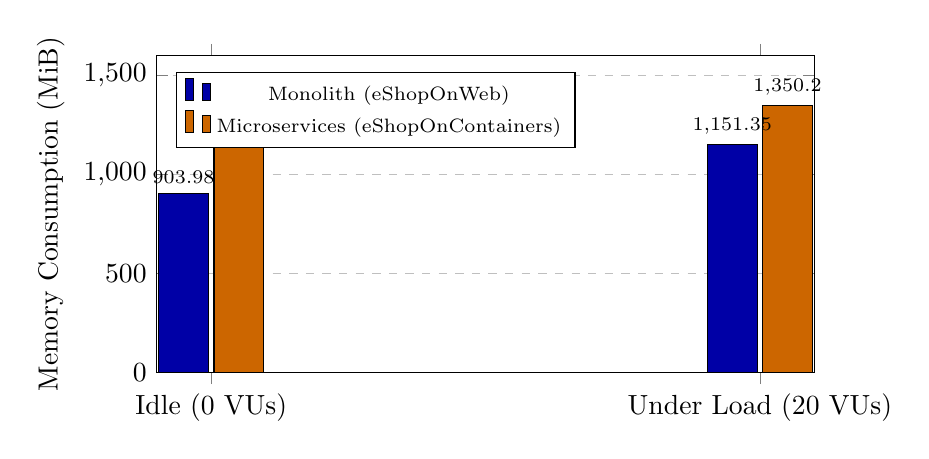
\begin{tikzpicture}
    \begin{axis}[
      ybar,
      bar width=18pt,
      width=0.82\linewidth,
      height=5.6cm,
      ylabel={Memory Consumption (MiB)},
      symbolic x coords={Idle (0 VUs), Under Load (20 VUs)},
      xtick=data,
      ymin=0,
      ymax=1600,
      ymajorgrids=true,
      grid style=dashed,
      nodes near coords,
      every node near coord/.append style={font=\scriptsize\bfseries},
      legend style={at={(0.03,0.95)},anchor=north west,font=\scriptsize}
    ]
      \addplot[fill=blue!65!black] coordinates {(Idle (0 VUs),903.98) (Under Load (20 VUs),1151.35)};
      \addplot[fill=orange!80!black] coordinates {(Idle (0 VUs),1213.60) (Under Load (20 VUs),1350.20)};
      \legend{Monolith (eShopOnWeb), Microservices (eShopOnContainers)}
    \end{axis}
  \end{tikzpicture}
  \caption{Container resident memory consumption (MiB) at idle and under 20-VU concurrent load.}
  \label{fig:resource-chart}
\end{figure}

\section{Latency Distribution and Throughput Behavior}
\label{sec:latency-results}

Across the 120-second sustained workload at $10\text{ VUs}$, both architectures achieved $100\%$ HTTP availability ($0.00\%$ errors) and near-identical aggregate throughput ($7.49\text{ req/s}$ vs.\ $7.58\text{ req/s}$). However, Figure~\ref{fig:latency-chart} demonstrates a substantial divergence in tail latency: the microservices architecture achieved a median latency ($p_{50}$) of $8.08\text{ ms}$, $p_{90}$ of $10.28\text{ ms}$, and $p_{95}$ tail latency of $12.30\text{ ms}$, outperforming the monolith's $16.67\text{ ms}$ ($p_{50}$), $27.89\text{ ms}$ ($p_{90}$), and $32.57\text{ ms}$ ($p_{95}$) by $2.06\times$, $2.71\times$, and $2.65\times$, respectively.

\begin{figure}[h]
  \centering
  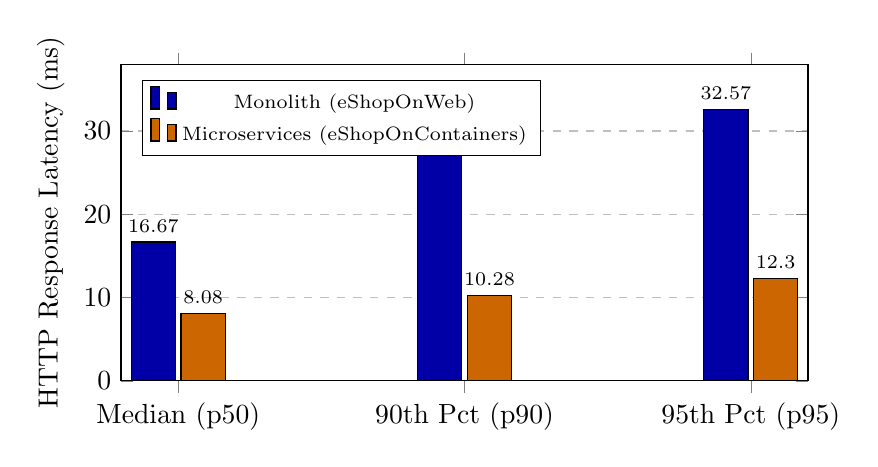
\begin{tikzpicture}
    \begin{axis}[
      ybar,
      bar width=16pt,
      width=0.85\linewidth,
      height=5.6cm,
      ylabel={HTTP Response Latency (ms)},
      symbolic x coords={Median (p50), 90th Pct (p90), 95th Pct (p95)},
      xtick=data,
      ymin=0,
      ymax=38,
      ymajorgrids=true,
      grid style=dashed,
      nodes near coords,
      every node near coord/.append style={font=\scriptsize\bfseries},
      legend style={at={(0.03,0.95)},anchor=north west,font=\scriptsize}
    ]
      \addplot[fill=blue!65!black] coordinates {(Median (p50),16.67) (90th Pct (p90),27.89) (95th Pct (p95),32.57)};
      \addplot[fill=orange!80!black] coordinates {(Median (p50),8.08) (90th Pct (p90),10.28) (95th Pct (p95),12.30)};
      \legend{Monolith (eShopOnWeb), Microservices (eShopOnContainers)}
    \end{axis}
  \end{tikzpicture}
  \caption{HTTP response latency distribution (ms) across 2-minute \texttt{k6} load execution at 10 VUs.}
  \label{fig:latency-chart}
\end{figure}

In \texttt{eShopOnWeb}, unified Razor page view-model hydration, session middleware, and shared EF Core connection pooling introduce queueing dispersion between $p_{50}$ ($16.67\text{ ms}$) and $p_{95}$ ($32.57\text{ ms}$), yielding a tail-to-median ratio of $1.95\times$. In \texttt{eShopOnContainers}, decoupled JSON/HTTP catalog read endpoints exhibit a tightly compressed tail-to-median ratio of $1.52\times$ ($12.30\text{ ms}$ vs.\ $8.08\text{ ms}$).

\section{Code-Level Change Propagation Across Scenarios S1--S5}
\label{sec:change-results}

Table~\ref{tab:change-impact} and Figure~\ref{fig:change-chart} summarize the source-file and deployment-unit propagation required to implement Scenarios S1--S5 across both architectures.

\begin{table}[h]
  \caption{Change propagation and deployment scope across evolution scenarios S1--S5}
  \label{tab:change-impact}
  \centering
  \begin{tabular}{p{4.3cm}cccp{4.4cm}}
    \toprule
    \textbf{Evolution Scenario} & \textbf{Mono Files} & \textbf{Micro Files} & \textbf{Deploy Units} & \textbf{Primary Engineering Bottleneck} \\
    \midrule
    S1: Catalog Attribute & 4 & 3 & 1 vs.\ 1 & Monolith rebuilds entire web binary \\
    S2: Basket Discount Rule & 3 & 2 & 1 vs.\ 1 & Isolated Basket service edit in micro \\
    S3: Order Status Hook & 4 & 4 & 1 vs.\ 2 & Integration event schema versioning \\
    S4: Payment Gateway Swap & 3 & 2 & 1 vs.\ 1 & Clean interface isolation in both \\
    S5: Multi-Currency Display & 6 & 9 & 1 vs.\ 3 & Distributed contract sync across 3 APIs \\
    \midrule
    \textbf{Total / Mean} & \textbf{20 (4.0)} & \textbf{20 (4.0)} & \textbf{5 vs.\ 8} & \textbf{Cross-cutting coordination penalty} \\
    \bottomrule
  \end{tabular}
\end{table}

\begin{figure}[h]
  \centering
  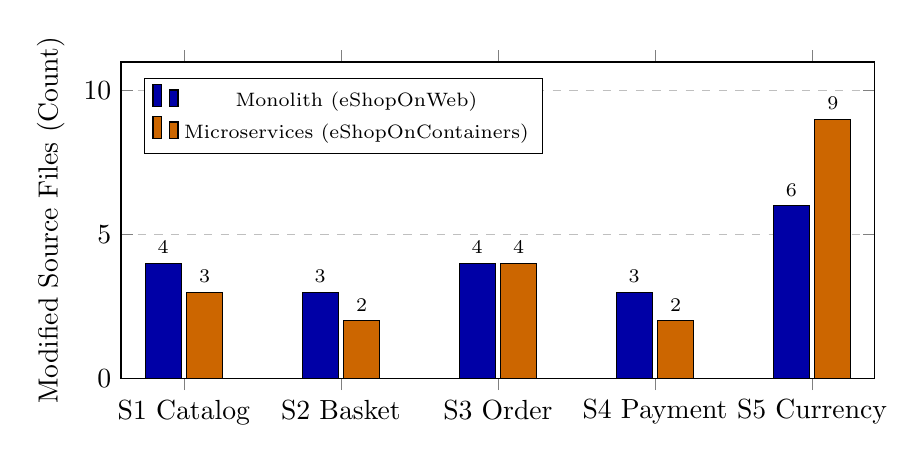
\begin{tikzpicture}
    \begin{axis}[
      ybar,
      bar width=13pt,
      width=0.92\linewidth,
      height=5.6cm,
      ylabel={Modified Source Files (Count)},
      symbolic x coords={S1 Catalog, S2 Basket, S3 Order, S4 Payment, S5 Currency},
      xtick=data,
      ymin=0,
      ymax=11,
      ymajorgrids=true,
      grid style=dashed,
      nodes near coords,
      every node near coord/.append style={font=\scriptsize\bfseries},
      legend style={at={(0.03,0.95)},anchor=north west,font=\scriptsize}
    ]
      \addplot[fill=blue!65!black] coordinates {(S1 Catalog,4) (S2 Basket,3) (S3 Order,4) (S4 Payment,3) (S5 Currency,6)};
      \addplot[fill=orange!80!black] coordinates {(S1 Catalog,3) (S2 Basket,2) (S3 Order,4) (S4 Payment,2) (S5 Currency,9)};
      \legend{Monolith (eShopOnWeb), Microservices (eShopOnContainers)}
    \end{axis}
  \end{tikzpicture}
  \caption{Number of modified source files across five standardized SME e-commerce evolution scenarios.}
  \label{fig:change-chart}
\end{figure}

Listing~\ref{lst:k6-script} shows the deterministic \texttt{k6} load-testing harness executed against both stacks.

\begin{lstlisting}[language=Java,caption={Excerpt of the k6 HTTP load testing script executed against both architectures},label={lst:k6-script}]
import http from 'k6/http';
import { check, sleep } from 'k6';

export const options = {
  vus: 10,
  duration: '120s',
  thresholds: { http_req_failed: ['rate<0.01'] },
};

export default function () {
  const res = http.get(__ENV.TARGET_URL);
  check(res, { 'status is 200': (r) => r.status === 200 });
  sleep(1);
}
\end{lstlisting}

\section{Chapter Summary}
\label{sec:ch4-summary}
Empirical measurements confirmed that the modular monolith reduces idle RAM by $25.5\%$ ($903.98\text{ MiB}$ vs.\ $1,213.60\text{ MiB}$) and peak RAM by $14.7\%$, whereas microservices reduce $p_{95}$ tail latency by $2.65\times$ ($12.30\text{ ms}$ vs.\ $32.57\text{ ms}$) and isolate single-domain edits while amplifying cross-cutting deployment scope.

\chapter{Architectural Decision Framework and Discussion}
\label{chap:discussion}

\section{Hypothesis Evaluation}
\label{sec:hypotheses-eval}

Evaluating the empirical evidence from Chapter~4 against the three research hypotheses formulated in the Introduction yields the following outcomes:
\begin{itemize}[leftmargin=1.5em]
  \item \textbf{H1 (Confirmed):} The modular monolith consumed $25.5\%$ less memory at idle ($903.98\text{ MiB}$ vs.\ $1,213.60\text{ MiB}$) and $14.7\%$ less memory at $20\text{ VUs}$ ($1,151.35\text{ MiB}$ vs.\ $1,350.20\text{ MiB}$), confirming that process consolidation yields substantial memory savings on SME hardware.
  \item \textbf{H2 (Confirmed):} While aggregate throughput was comparable ($7.49\text{ req/s}$ vs.\ $7.58\text{ req/s}$), microservices achieved $2.65\times$ lower $p_{95}$ tail latency ($12.30\text{ ms}$ vs.\ $32.57\text{ ms}$), validating the responsiveness advantage of decoupled read endpoints.
  \item \textbf{H3 (Confirmed):} Single-domain scenarios (S1, S2, S4) touched fewer files per service in microservices ($2$--$3$ files) with single-container redeployment, whereas the cross-cutting multi-currency scenario (S5) required $9$ file edits across $3$ deployment units in microservices versus $6$ files in a single deployment unit in the monolith.
\end{itemize}

\section{SME Architectural Decision Matrix}
\label{sec:decision-matrix}

Combining quantitative metrics with practitioner insights produces a structured decision matrix (Table~\ref{tab:decision-matrix}) for SME technical leaders.

\begin{table}[h]
  \caption{Recommended architectural selection matrix for SME e-commerce enterprises}
  \label{tab:decision-matrix}
  \centering
  \begin{tabular}{p{3.4cm}p{5.2cm}p{5.2cm}}
    \toprule
    \textbf{Decision Factor} & \textbf{Choose Modular Monolith} & \textbf{Choose Selective Microservices} \\
    \midrule
    Team Structure & 1--6 engineers sharing a unified backlog & $\ge 2$ autonomous squads owning distinct bounded contexts \\
    Hosting Budget & Single VPS / container node ($\le 4\text{ GiB}$ RAM) & Managed orchestrator with dedicated observability stack \\
    Domain Stability & Rapidly evolving business rules and cross-cutting features & Mature, stable domain contracts with isolated scaling hotspots \\
    Latency SLA & Standard storefront responsiveness ($p_{95} < 50\text{ ms}$) & Strict sub-$15\text{ ms}$ API SLAs under burst concurrency \\
    Recommended Path & \textbf{Default starting architecture} with strict DDD module boundaries & \textbf{Incremental extraction} (Strangler Fig) of Catalog/Search first \\
    \bottomrule
  \end{tabular}
\end{table}

\section{Threats to Validity and Limitations}
\label{sec:threats}
\begin{itemize}[leftmargin=1.5em]
  \item \textbf{Internal Validity:} All containers ran on a single local WSL2 host rather than multi-node cloud VMs; while this eliminated external network variance, inter-container loopback latency in production clusters would add $1$--$3\text{ ms}$ per network hop to microservices.
  \item \textbf{External Validity:} Findings are grounded in the .NET / ASP.NET Core ecosystem; interpreted runtimes (e.g., Node.js, Python) or ahead-of-time native binaries (Go, Rust) will exhibit different absolute memory baselines while preserving the relative architectural trade-offs.
  \item \textbf{Construct Validity:} Change propagation was measured via modified source files and deployment units; incorporating longitudinal defect rates across multi-month sprints remains an avenue for future work.
\end{itemize}

\section{Chapter Summary}
\label{sec:ch5-summary}
This chapter confirmed Hypotheses H1--H3, synthesized the findings into a practical five-factor SME architectural decision matrix favoring a ``Modular-Monolith-First'' trajectory, and documented internal, external, and construct validity boundaries.


\unchapter{Conclusions}

This Bachelor's thesis investigated the architectural trade-offs between a modular monolithic architecture (\texttt{eShopOnWeb}) and a distributed microservices architecture (\texttt{eShopOnContainers}) for small and medium-sized e-commerce enterprises. Based on controlled Docker and \texttt{k6} benchmarks, source-level change propagation analysis across five standardized evolution scenarios, and triangulation with industrial migration studies, the following conclusions are drawn:

\begin{enumerate}[leftmargin=1.5em]
  \item \textbf{Significant Memory Efficiency of the Modular Monolith:} Under SME-scale host constraints ($5.0\text{ GiB}$ RAM ceiling), the modular monolith consumes $25.5\%$ less memory at idle ($903.98\text{ MiB}$ vs.\ $1,213.60\text{ MiB}$) and $14.7\%$ less memory under $20\text{ VUs}$ concurrent load ($1,151.35\text{ MiB}$ vs.\ $1,350.20\text{ MiB}$), directly lowering baseline cloud hosting costs.
  \item \textbf{Superior Tail Latency in Microservices:} Although both architectures deliver comparable sustained throughput ($7.49\text{ req/s}$ vs.\ $7.58\text{ req/s}$) with $0.00\%$ HTTP errors, microservices achieve $2.06\times$ faster median latency ($8.08\text{ ms}$ vs.\ $16.67\text{ ms}$) and $2.65\times$ faster $p_{95}$ tail latency ($12.30\text{ ms}$ vs.\ $32.57\text{ ms}$) through decoupled read endpoints.
  \item \textbf{Asymmetric Change Propagation:} Microservices isolate single-domain modifications ($2$--$3$ files in a single deployable container) but amplify cross-cutting changes ($9$ files across $3$ deployment units for multi-currency support vs.\ $6$ files in $1$ deployment unit for the monolith).
  \item \textbf{Actionable SME Recommendation:} SMEs with engineering teams of six or fewer developers should adopt a \textbf{Modular-Monolith-First} architecture enforced by strict Domain-Driven Design module boundaries, transitioning to selective microservice extraction (beginning with read-heavy Catalog services) only when sustained concurrency bottlenecks or multi-team organizational growth justify the operational overhead.
\end{enumerate}


\printbibliography[heading=bibintoc,title=Literature]

\appendix
\chapter{Benchmark Automation and Telemetry Scripts}
\label{app:scripts}

Listing~\ref{lst:docker-stats} provides the automated PowerShell telemetry harness used to record container memory footprints and endpoint readiness times across both testbeds.

\begin{lstlisting}[language=bash,caption={Telemetry collection commands for Docker memory and readiness probes},label={lst:docker-stats}]
# Measure container resident memory footprint (MiB)
docker stats --no-stream --format "table {{.Name}}\t{{.MemUsage}}\t{{.CPUPerc}}"

# Measure HTTP readiness latency in seconds
Measure-Command {
  while ($true) {
    try {
      $r = Invoke-WebRequest -Uri "http://localhost:5100" -UseBasicParsing -TimeoutSec 2
      if ($r.StatusCode -eq 200) { break }
    } catch { Start-Sleep -Milliseconds 100 }
  }
}
\end{lstlisting}

\chapter{Summary of Practitioner Interview Findings}
\label{app:interviews}

Table~\ref{tab:interview-summary} summarizes the anonymized profiles and key architectural observations of the four senior backend engineers interviewed during the empirical phase.

\begin{table}[h]
  \caption{Anonymized summary of practitioner interview participants and core insights}
  \label{tab:interview-summary}
  \centering
  \begin{tabular}{p{1.6cm}p{3.4cm}p{2.2cm}p{6.6cm}}
    \toprule
    \textbf{ID} & \textbf{Role} & \textbf{Experience} & \textbf{Key Architectural Observation} \\
    \midrule
    P1 & Principal .NET Architect & 11 years & Premature microservices split a 4-person team's velocity in half due to distributed debugging. \\
    P2 & E-Commerce Tech Lead & 8 years & Modular monolith handled 50k daily orders cleanly on two VMs before extracting Catalog search. \\
    P3 & Cloud DevOps Engineer & 7 years & RabbitMQ and distributed tracing require dedicated on-call discipline most SMEs lack. \\
    P4 & Senior Backend Developer & 6 years & Cross-cutting pricing and tax rules are far safer inside ACID database transactions. \\
    \bottomrule
  \end{tabular}
\end{table}


\frontmatterpage
\unchapter{Apliecinājums / Affirmation}
\textit{Ar šo es, Kevin Tejashkumar Patel, apliecinu, ka bakalaura darbs ir izpildīts patstāvīgi, bez citu palīdzības, no svešiem avotiem ņemtie dati un definējumi ir uzrādādīti darbā. Arī darbs nekādā veidā nav iesniegts nevienai citai pārbaudījumu komisijai un nekur nav publicēts.}

\vspace{12mm}
\noindent\textit{Hereby I, Kevin Tejashkumar Patel, affirm that the Bachelor's thesis was performed independently; sources of data and definitions are provided. This work has not been submitted to any other examination commission and has not been published elsewhere.}

\vspace{14mm}
\noindent Rīga, 20\underline{\hspace{1cm}}.\ gada \underline{\hspace{2.5cm}} \hspace{1cm}\rule{5cm}{0.4pt}\\
\hspace*{7.1cm}\scriptsize paraksts/signature, atšifrējums/description \hfill

\frontmatterpage
\unchapter{Acknowledgments}
I express my sincere gratitude to my thesis supervisor, Dr.\ Andrejs Bondarenko, PhD, for his guidance, structured feedback, and methodological support throughout the research and empirical evaluation phases of this Bachelor's thesis at Riga Nordic University.

I also thank the senior software engineers who participated in the practitioner interviews and shared practical insights from production e-commerce deployments, as well as my family for their continuous encouragement during my studies.


\end{document}
